\section{Durchführung}
\label{sec:Durchführung}

\begin{figure}
  \centering
  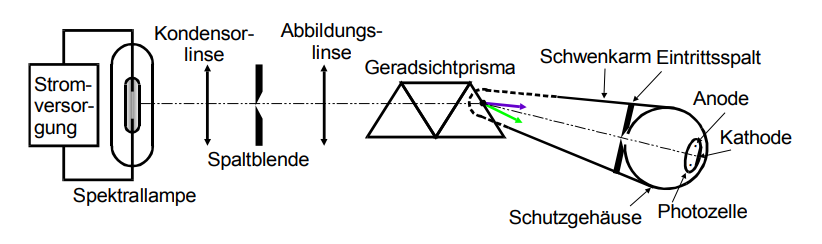
\includegraphics[width=0.95\textwidth]{content/ver-aufbau.png}
  \caption{Anordnung der optischen und elektrischen Elemente zur Untersuchung des Photoeffekts \cite{V500}.}
  \label{fig:ver-aufbau}
\end{figure}

Zunächst werden die einzelnen Elemente gemäß \autoref{fig:ver-aufbau} aufgestellt.
Das Licht, welches durch die Kondensorlinse kommt, wird so auf dem Spalt gebündelt, dass das Bild dieselbe Größe wie der Spalt hat.
Die Abbildungslinse wird so verschoben, dass an der Photozelle ein scharfes Bild zu sehen ist.
Das Prisma fächert die Strahlen so auf, dass mit der Photozelle genau eine Spektrallinie aufgenommen werden kann.
Als Spektrallampe wird in diesem Versuch eine Quecksilberdampflampe genutzt.

Zunächst wird für die verschiedenen zu sehenden Spektrallinien der Photostrom gemessen,
während die Gegenspannung variiert wird. Die Messung wird beendet, sobald der Photostrom auf 0 A absinkt.
Es ist weiterhin darauf zu achten, dass zu jeder Linie mindestens 10 Messwerte aufgenommen werden.

Im letzten Versuchsteil wird die Photozelle auf der gelben Spektrallinie ($\lambda = 577$ nm) ausgerichtet.
Nun wird die Gegenspannung von -20 V bis +20 V geregelt und der jeweilige Photostrom notiert.
